\documentclass[11pt, margin=1in]{article}
\usepackage{amsmath}
\usepackage{amsfonts}
\usepackage{amssymb}
\usepackage[margin=1in]{geometry}
\usepackage{fancyhdr}
\usepackage{natbib}
\usepackage{hyperref}

\hypersetup{
    colorlinks=true,
    citecolor=blue,
    urlcolor=red
}

% Use these for theorems, lemmas, proofs, etc.
\newtheorem{theorem}{Theorem}
\newtheorem{lemma}[theorem]{Lemma}
\newtheorem{proposition}[theorem]{Proposition}
\newtheorem{claim}[theorem]{Claim}
\newtheorem{corollary}[theorem]{Corollary}
\newtheorem{definition}[theorem]{Definition}
\newtheorem{fact}[theorem]{Fact}
\usepackage{tikz}
\usetikzlibrary{arrows}
\newenvironment{proof}{\noindent {\it Proof.}}{\hfill\rule{2mm}{2mm}}
\pagestyle{fancy}
\lhead{\textbf{CS236r Project Proposal}}
\rhead{\textit{Alex Lin \& Melissa Yu}}
\cfoot{\thepage}
\renewcommand{\headrulewidth}{0.4pt}
\renewcommand{\footrulewidth}{0.4pt}
\newcommand{\card}[1]{\ensuremath{\left\vert#1\right\vert}}
\newcommand{\diff}[1]{\, d#1}
\newcommand{\eval}[2]{\Big|_{#1}^{#2}}

\makeatletter

\begin{document}
	
\title{CS236r Project Update \\ Scoring Systems for Predicting Credit Risk}
\author{Alex Lin \and Melissa Yu}
\date{}
\maketitle

\section{Introduction}
In our final project, we apply the  Supersparse Linear Integer Model (SLIM) scoring system to make interpretable predictions of loan default risk. We begin by examining a simple neural network baseline model, which achieves reasonably high accuracies on our dataset, but falls short in terms of both interpretability and fairness, two important requirements for any credit scoring model. We then describe TODO

\section{Baseline}
Benchmark studies of classification algorithms for credit scoring discuss these models in the framework of both individual (e.g., CART, Linear support vector machine, Logistic Regression, Multilayer perceptron artificial neural network) and ensemble methods (e.g, Bagged decision trees, Simple average ensemble). To gain a preliminary gauge of the performance of a simple model on our dataset, we explore the use of Multilayer perceptron artificial neural networks.

\subsection{Data} 
We use the GMC dataset, which was provided by a financial institution for the ``Give me some credit'' Kaggle competition (\url{https://www.kaggle.com/c/GiveMeSomeCredit}). This comprises historical data on 250,000 borrowers, each quantified along 10 dimensions, including age and monthly income. Notably, this dataset does not include information on the borrowers' race or gender. We are considering using the German credit (GC) dataset from the UCI Library (Lichman, 2013) for future work, since it does include these features and may allow us to quantify fairness more accurately.

\subsection{Neural Network Model} 
We used PyTorch to implement a single-layer, linear, feedforward neural net with hidden layer size 30 and ReLU activations. The model was trained using the Adam optimizer with learning rate 0.0001 over 30 epochs. Our vanilla model achieved an AUC score of 0.801831 on the Kaggle test set. However, while this model has reasonable predictive power, is not very interpretable to consumers: The model's classification process cannot be easily explained to or understood by consumers, and neither can the most important predictive factors can be
intuitively identified to aid loan seekers in improving their profile. 

This baseline also has low fairness: As discussed in our project proposal, the model must comply with the Equal Credit Opportunity Act (ECOA) and Fair Credit Reporting Act (FCRA). Thus, it cannot discriminate on the basis of race, age, education, employment history, gender, marital status, or wealth. We perform a rudimentary evaluation of the group fairness of our classification model by visualizing the population age distribution and the age distribution of borrowers predicted to default on the same histogram. The two distributions diverge quite a bit, with the percentage of young people predicted to default being much higher than the percentage of young people in the population as a whole. This indicates our algorithm may not be fair when it comes to age.

\begin{center}
	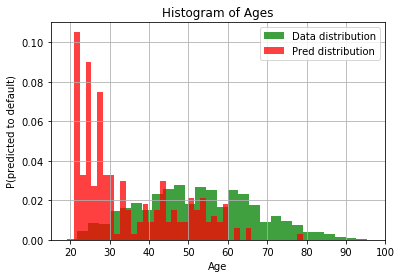
\includegraphics[width=0.9\linewidth]{age-fairness}
\end{center}

\section{Research Proposal}

\end{document}